\section{高维最小绝对值回归的性能研究}

本文的主题是$L_1$范数稳健方法在宏观经济中的应用问题研究。
$L_1$范数是最常用的几种重要范数之一,它在数值计算、统计学、运筹学、
机器学习等领域有着极为重要的应用。在统计学研究中,已经基于$L_1$范数发展出了许多
稳健统计方法,主要是利用$L_1$范数的良好统计性质。

$L_1$范数稳健方法在计量经济学中已有广泛应用,
其中一个重要应用就是最小绝对值回归。最小绝对值回归最早提出是为了弥补最小二乘法的不足。
使用最小二乘法建立的线性回归模型虽然具有较好的解释性,
但是高斯——马尔可夫条件对模型变量的分布有正态性的要求。因此直接使用最小二乘法来建立模型,往往
对原始数据的分布情况要求高。即使变量满足了正态分布,但在模型系数估计时,样本中离群值的存在对
模型的系数估计效果有很大影响。

在宏观经济实证研究中,经济变量一般
不能够服从正态分布,而因受到经济冲击呈现出重尾的特征。对这样的原始数据不能够通过最小二乘法直接建模,
因此常常在回归中剔除异常点,使得经济变量接近正态分布,然而代价是有可能损失较多有价值的信息。

采用最小绝对值回归,是更加稳健的做法。实质上它就是中位数回归,模型的系数也具有很好的解释意义,
已经广泛应用在对居民收入的研究中,并且在金融数据分析领域有着广泛的应用。
在模型的拟合上,最小绝对值回归对离群值不敏感,具有相当的稳健性,因此可以很好处理重尾的宏观经济变量。

高维宏观经济数据,往往包含了维数众多的经济变量,并且样本数量往往非常大,
此时如果想要直接使用最小绝对值回归,在求解时就
需要解决变量维数和约束数量很高的线性规划问题,因此计算的开销很高。

最小绝对值回归在计算上的复杂性在一定程度上限制了它的应用。
一直以来,普遍的加速最小绝对值回归的方法都尝试使用平滑化方法来近似最小绝对值回归的目标函数,
避免直接使用原目标函数。然而,替换目标函数,可能会影响估计量的一致性从而
影响最小绝对值回归模型的解释性。

但是近年来随着统计学和机器学习领域
对$L_1$范数的研究逐渐深入,不断有新的算法尝试解决这个问题。
本章将介绍最小绝对值回归的两种较新的估计算法,一种是基于聚类——迭代拆解的算法;
另一种是基于替代变量的牛顿迭代方法,两种算法基于不同的出发点,
都在一定程度上对解决最小绝对值回归问题做了优化。

\subsection{简介}
\subsubsection{$L_1$范数的稳健性}

$L_2$范数最优化问题最常见的是最小二乘法。
最小二乘法的优点很多,这里不赘述。尽管在求解大部分问题时用最小二乘估计求解可以得到比较令人满意
的效果, 但最小二乘法也存在一些局限性, 比如, 当收集的数据较少或者具有较多的缺失数据
并且数据中夹杂有异常点时, 用最小二乘法所得的结果就令人难以接受, 在此情况下应用所得到到的回归方程或模型进行预测或者拟合时, 
则预测或拟合的精度是相当低的, 甚至根本不能使用。正因为最小二乘法对数据中的异常值十分敏感,当数据中具有较多离群值时,通过最小二乘、PCA和SVD方法,得到的估计结果也会受到较大影响。

这里可以不使用最小二乘法而选择$L_1$范数的方法即最小一乘法,它可以增加估计的健壮性。
设$\bm{X} = (X_1, X_2, ..., X_p)^T$为一$p$维随机变量,$Y$为响应变量,$\bm{\beta}$为回归系数。
假设我们观察到$i.i.d. $样本$\bm{X}_{n\times p} = (\bm{x}_1, \bm{x}_2, ..., \bm{x_n})^T$和$\bm{Y}_{n\times1}=
(y_1, ..., y_n)^T$,我们一般使用$\bm{\beta}$
的最小二乘估计量
\begin{equation}\label{l2loss}
\hat{\bm{\beta}} = \underset{\bm{\beta}}{\operatorname{arg\ min}} \sum_{i=1}^n\|y_i - \bm{x}^T_i\bm{\beta}\|_{L_2}
=\underset{\bm{\beta}}{\operatorname{arg\ min}} \sum_{i=1}^n(y_i - \bm{x}^T_i\bm{\beta})^2
\end{equation}
在稳健统计中,我们经常使用其他的目标函数,例如使用$L_1$范数来代替$L_2$,

\begin{equation}\label{l1loss}
\hat{\bm{\beta}} = \underset{\bm{\beta}}{\operatorname{arg\ min}} \sum_{i=1}^n\|y_i - \bm{x}^T_i\bm{\beta}\|_{L_1}
=\underset{\bm{\beta}}{\operatorname{arg\ min}} \sum_{i=1}^n|y_i - \bm{x}^T_i\bm{\beta}|
\end{equation}
如图所示,通常使用$L_1$范数在线性回归中可以有效避免离群值造成的干扰。
\begin{figure}[H]
    \centering
    \begin{minipage}[t]{0.48\textwidth}
    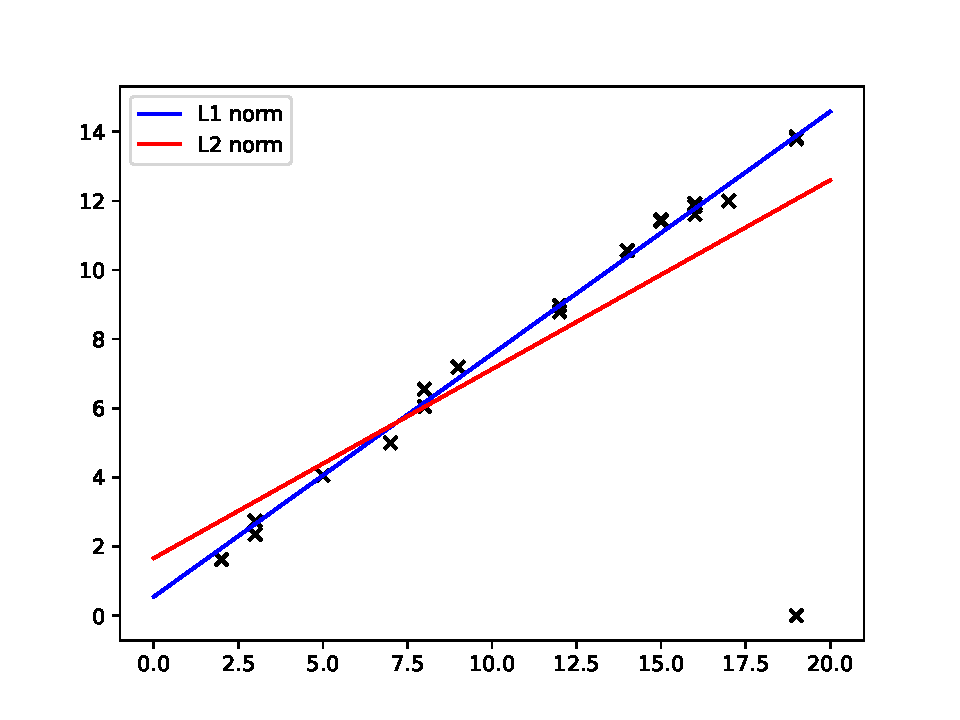
\includegraphics[width=8cm]{pics/chapter2/l1-l2-diff2.pdf}
    \end{minipage}
    \begin{minipage}[t]{0.48\textwidth}
    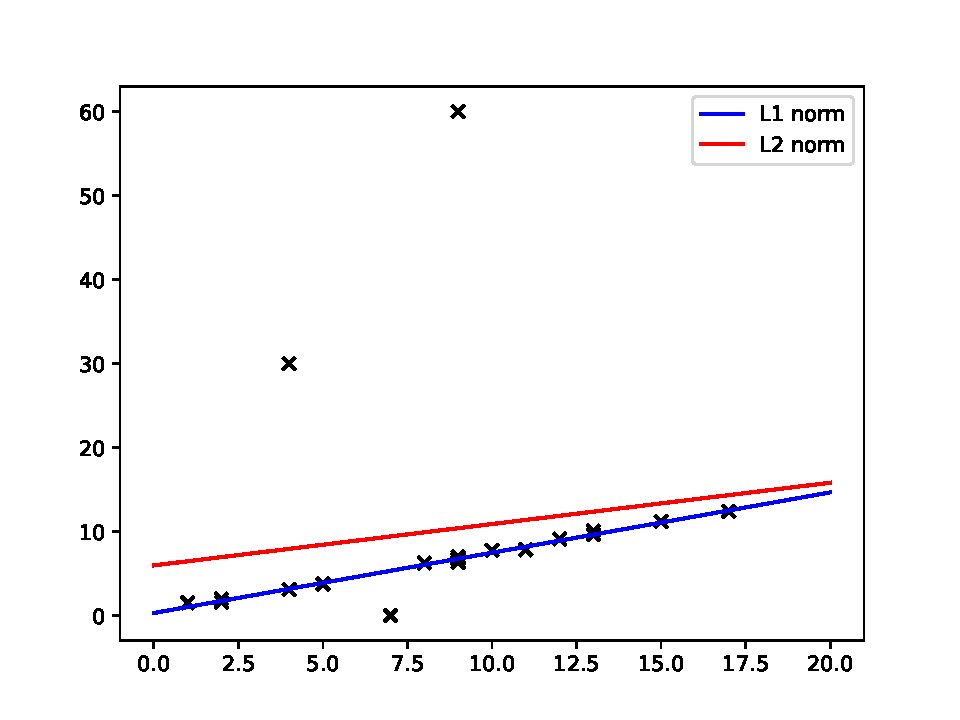
\includegraphics[width=8cm]{pics/chapter2/l1-l2-diff.pdf}
    \end{minipage}
    \caption{\small 如图所示,在简单的线性模型的拟合中,出现一个离群值就可以导致最小二乘法拟合出现明显的偏差;
    而含有较多离群值时最小二乘法拟合变得很不可靠;而采用$L_1$范数则具有相当稳健性。}
    \label{fig2.1}

\end{figure}

我们使用$L_1$目标函数来估计$\bm{\beta}$,则其中$\bm{\beta}^*$为最小绝对值回归系数,$e$为一随机噪声,
可以写出最小绝对值回归的一般形式
\begin{equation} \label{l1losstotal}
    \begin{split}
    Y &= \bm{X}^T\bm{\beta}^* + e\\
    \bm{\beta}^* &= \underset{\bm{\beta}\in \mathbb{R}^{p}}{\operatorname {arg\ min}}
    \mathbb{E}|Y - X\bm{\beta}|.
    \end{split}
\end{equation}

\subsubsection{最小绝对值回归的估计方法}
对于\eqref{l1loss},它是一个凸优化问题,但是其不具备显式解,一般求它的数值解。但是其目标函数在$\bm{0}$点不可导,
因此不能直接使用使用梯度下降法,一般来说,该问题
的全局最优解可以通过求解下面的线性规划问题得到:
$$
    \underset{\bm{\beta}, \bm{t}}{\operatorname{min\ }} 1^T \bm{t}
$$
$$
    s.t. -\bm{t} \leq \bm{X}_{n\times p}\bm{\beta}_{p\times1} - \bm{Y}_{n\times 1} \leq \bm{t}
$$
目前对于线性规划问题已经有了比较成熟的解决方法,主要通过单纯形法或者内点法求解,后者的时间复杂度可以控制在多项式时间,
然而,一般而言,当$n$和$p$均很大时,上述线性规划问题面临很高的变量和约束维数,计算速度仍较慢。

由于$L_1$范数的目标函数在机器学习领域的大量使用,已经产生了一些光滑化方法,做法是用一个接近$L_1$的目标函数来替代它,
用来替代的函数往往处处可导,因而可以使用梯度下降法求解。
典型的代表就是使用Huber’s M统计量近似$L_1$范数目标函数,
\begin{equation*}
    \rho(e) = \left\{
        \begin{array}{clr}
            \frac1{2}e^2,\ |e| \leq \gamma \\
            \gamma |e| - \frac1{2}\gamma ^2 ,\ |e| > \gamma
        \end{array}
    \right.
\end{equation*}
其中$\gamma$为某一正数,该问题可以转化为一个二次规划问题求解。

\subsection{聚类——迭代拆解算法}
近年来针对最小绝对值回归的性能研究发展出了除了光滑化目标函数之外的方法,可以在不改变目标函数的情况下,
通过寻求新的优化方法进行求解。这样一来,可不改变最小绝对值回归估计量的统计性质。
这里介绍Park等人于2016年提出的一种基于聚类——迭代拆解算法的最小绝对值回归求解方法。

\subsubsection{聚类——迭代拆解算法说明}
聚类是一种在机器学习中常见的做法,就是按照某种给定的规则,将特征接近的样本点归类到一起。
聚类——迭代拆解算法的提出受到以下事实的启发:
1)优化问题规面临的数据集模庞大,其中许多的样本点在进行参数估计时的贡献是很接近的;
2)如果对相似的样本点进行聚类,提炼该聚类中的信息,避免每个样本点都进入计算,那么就会大大减小问题的规模;
3)假设在聚类后构造的新数据集上不能接近问题的最优解,那么就拆解当前的聚类,在新聚类上进行计算,
聚类个数有限,因此最坏情况下相当于直接求解原问题;

采用聚类——迭代拆解算法求解某个优化问题的前提如下:1)必须能够提出一种规则来对样本点聚类;
2)必须找到合适的聚类和拆解聚类的标准;
3)需要在聚类后构造的新数据集上明确定义新的优化问题;
4)能够判定当前解是否接近最优解。

算法2.1给出了任何一个聚类——迭代拆解算法的主要步骤,注意算法2.1必然在某处停止,
因为每次不断拆解聚类,当聚类个数$|K^{t}|= n$时,相当于计算原问题,此时算法终止。
\begin{table}[H]%%%%%%开始表格
    \centering%把表居中
    \begin{tabular}{{p{0.9\columnwidth}}}%三个c代表该表一共三列,内容全部居中
    
    \toprule%第一道横线 表头
    算法2.1:聚类——迭代拆解算法(Aggregate and Iterative Disaggregate, AID) \\
    \midrule%第二道横线 符号+解释+单位 中间用&隔开
    输入:原始数据集$\bm{X}_{n\times p}$,样本点的下标集合${I} = \{1, 2, ..., n\}$,
    数据的特征下标集合${J} = {1, 2, ..., p}$,原优化问题$P$。\\
    初始化:对原始数据集$\bm{X}$聚类,然后按某种规则产生新的优化数据集$\bm{X}^{1}$。 \\
    对于$t = 1, ..., T$:\\
        记${C}^{t} = \{{C}_1^{t}, ..., C_K^{t}\}$为聚类的集合, $K^t = {1, ..., |K^t|}$为当前聚类的下标,
        \\
        1.根据当前聚类情况${C}^{t}$,构造新的数据集$\bm{X}^{t}$,求解相应的优化问题${P}^{t}$; \\
        2.检查解$\bm{s}^{t}$是否达到最优条件;\\
        3.如果不满足条件,拆解当前聚类。
        \\
    \bottomrule%第三道横线
    \end{tabular}
\end{table}%%%%%%结束表格

\subsubsection{优化最小绝对值回归}
改写\eqref{l1loss}的目标函数,
\begin{equation}\label{l1loss2}
E^* = \underset{\bm{\beta} \in \mathbb{R}^{p}}{\operatorname{min}} 
\sum_{i \in I}|y_i - \sum_{j \in J}x_{ij}\bm{\beta}_j|
\end{equation}

首先给出聚类方法。给定$|K_0|$为目标聚类个数,初始化$C_0 = \{C_1^0, C_2^0, ..., C_K^0\}$,
我们可以使用任意的聚类方法进行初始化。接下来给出如何根据聚类来产生新的数据集,
对于在任一迭代周期内产生的聚类$C^t_k, k = 1, ..., K^t$,取
\begin{equation*}
    x_{kj}^t = \frac{\sum_{i \in C_k^t}x_{ij}}{|C_k^t|},\ j \in J \  
    \text{并且} \
    y_{k}^t = \frac{\sum_{i \in C_k^t}y_i}{|C_k^t|}
\end{equation*}

对于每一个不同的聚类需要给出一个权重来区分信息量不同的聚类,因此在新的数据集上,我们求解下面的问题
\begin{equation}\label{clusterl1}
    F^t =\underset{\bm{\beta}^t \in \mathbb{R}^{p}}{\operatorname{min}} 
    \sum_{k=1}^{K^t}|C_k^t||y_k^t - \sum_{j \in J}x_{kj}^t\bm{\beta}_j^t|
\end{equation}
容易发现,任何\eqref{clusterl1}的可行解都是\eqref{l1loss2}的可行解。
记$\hat{\bm{\beta}^t}$为\eqref{clusterl1}的解,在每次迭代,我们计算此时的原目标函数的取值
\begin{equation}
    E^t = \sum_{i \in I} |y_i - \sum_{j \in J}x_{ij}\hat{\bm{\beta}}_j^t|
\end{equation}

接下来给出拆解聚类的准则:设$t$步的聚类集合为$C^{t}$,该步解为$\hat{\bm{\beta}}_t$,
对于$k = 1, ..., K^t$,计算$\theta_i = y_i - \sum_{j \in J}x_{ij}\hat{\bm{\beta}}_j^t$,
1)若对于任意$i \in C_k^t$,$\theta_i$有相同的符号,那么该聚类$C^t_k$将保留到下次迭代,即$C^{t+1} \leftarrow C^{t+1}\bigcup C^t_k$,见图
\ref{aid-demo};

2)若不满足上述条件,那么根据$\theta_i$符号异同,将$C^t_k$分成两个集合,$C_{k+}^t = \{i \in C_k^t | \theta_i > 0\}$ ,
$C_{k-}^t = \{i \in C_k^t | \theta_i < 0\}$,见图\ref{aid-demo}b,这两个集合在下一步形成新的聚类,
即$C^{t+1} \leftarrow C^{t+1}\bigcup \{ C_{k+}^t, C_{k-}^t\}$,见图\ref{aid-demo}c。

\begin{figure}[H]
    \centering
    \begin{subfigure}[t]{0.3\textwidth}\label{aid-demo1}
    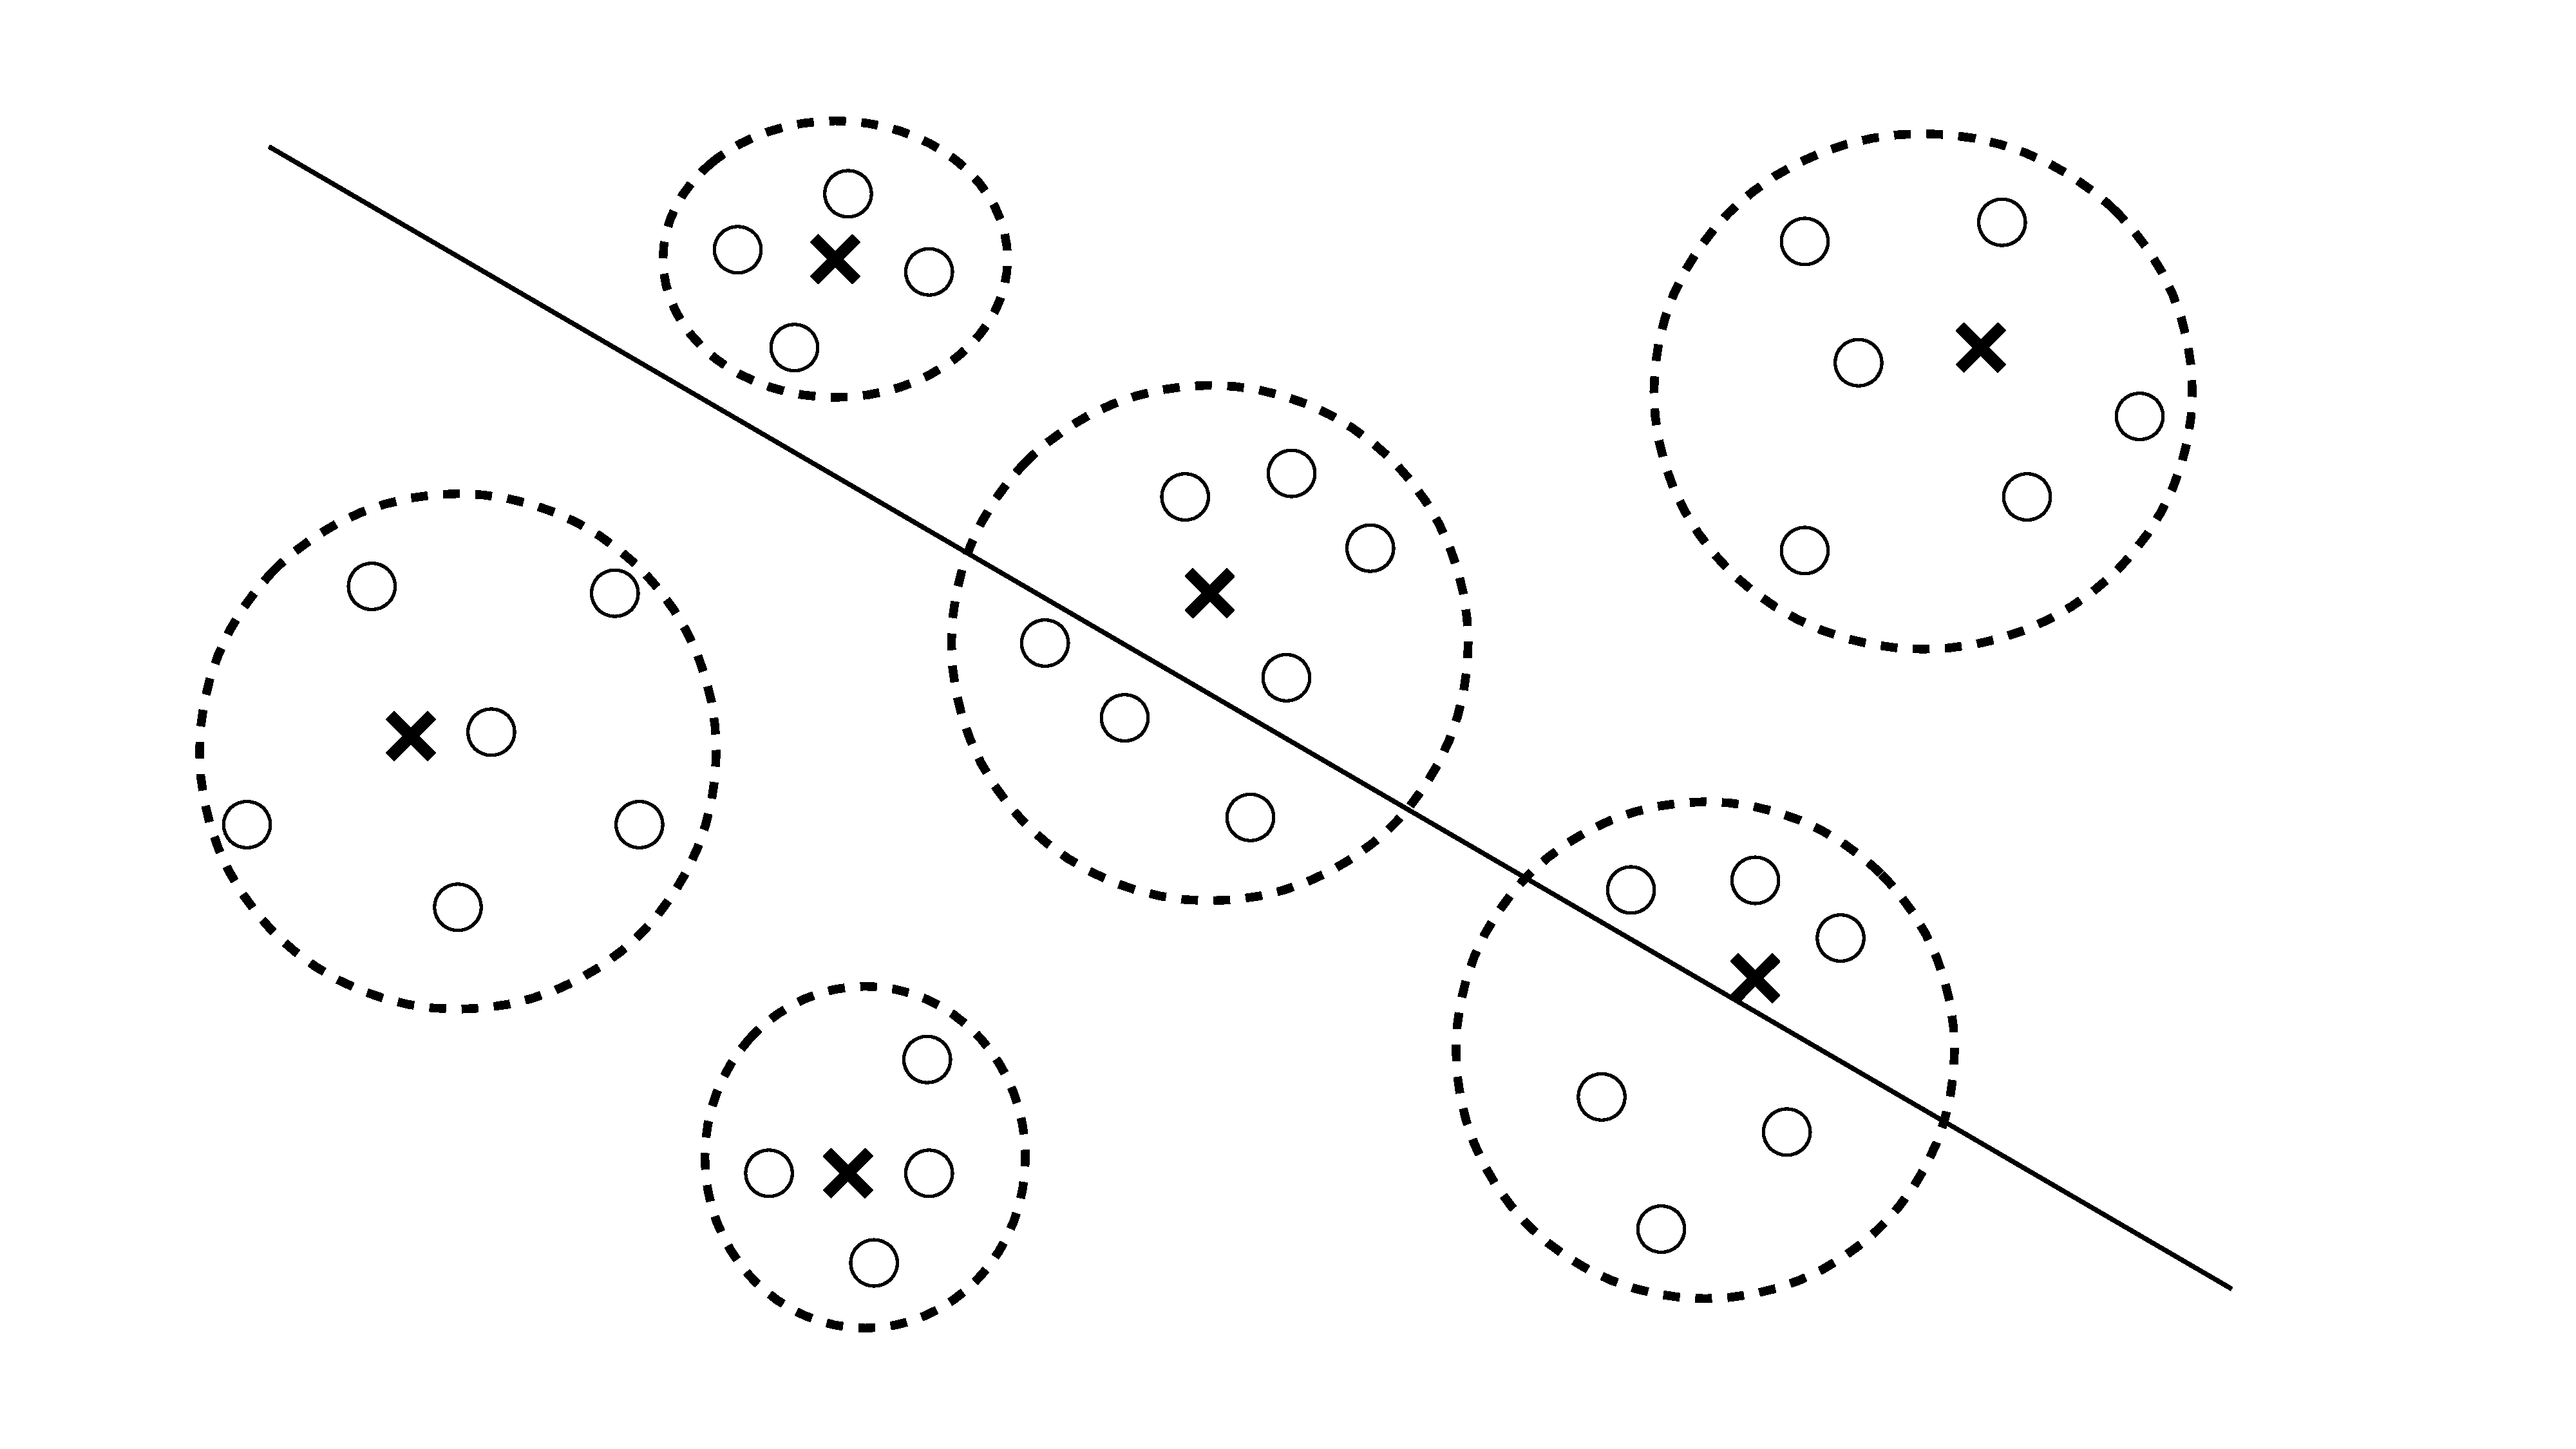
\includegraphics[width=6cm]{pics/chapter2/aid-demo-a.pdf}
    \captionof{figure}{}
    \end{subfigure}
    \begin{subfigure}[t]{0.3\textwidth}\label{aid-demo2}
    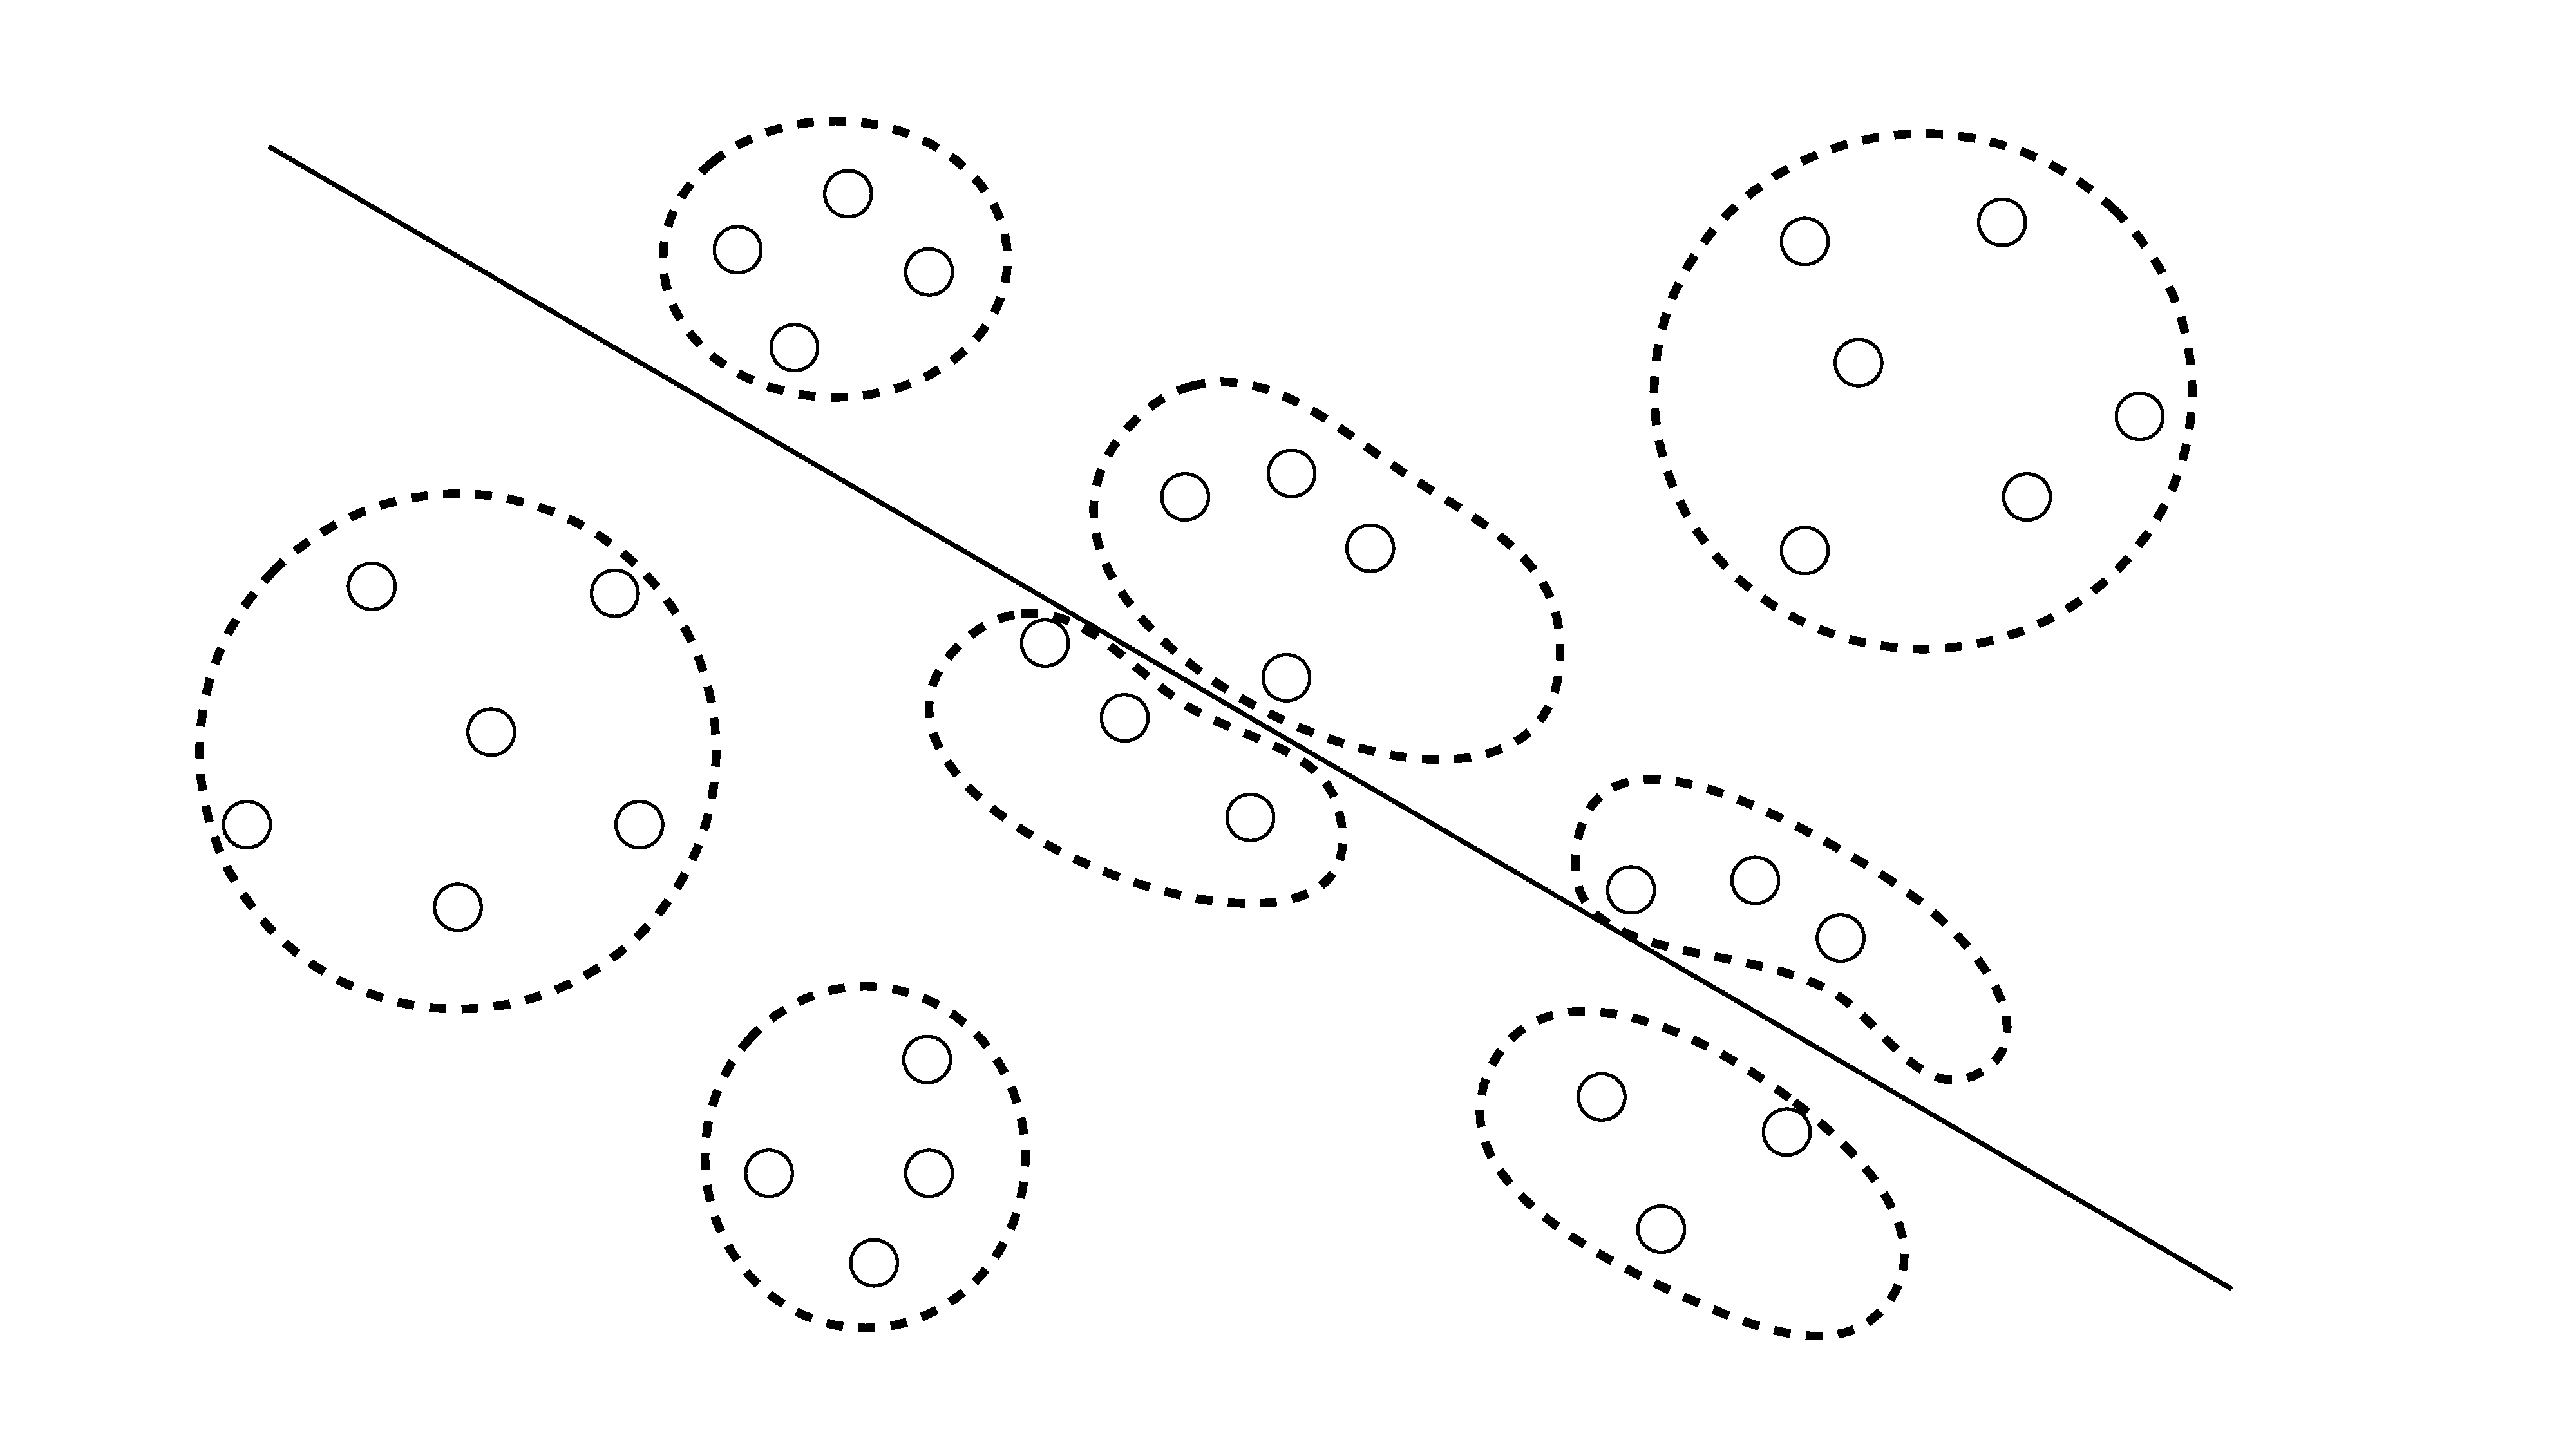
\includegraphics[width=6cm]{pics/chapter2/aid-demo-b.pdf}
    \captionof{figure}{}
    \end{subfigure}
    \begin{subfigure}[t]{0.3\textwidth}\label{aid-demo3}
    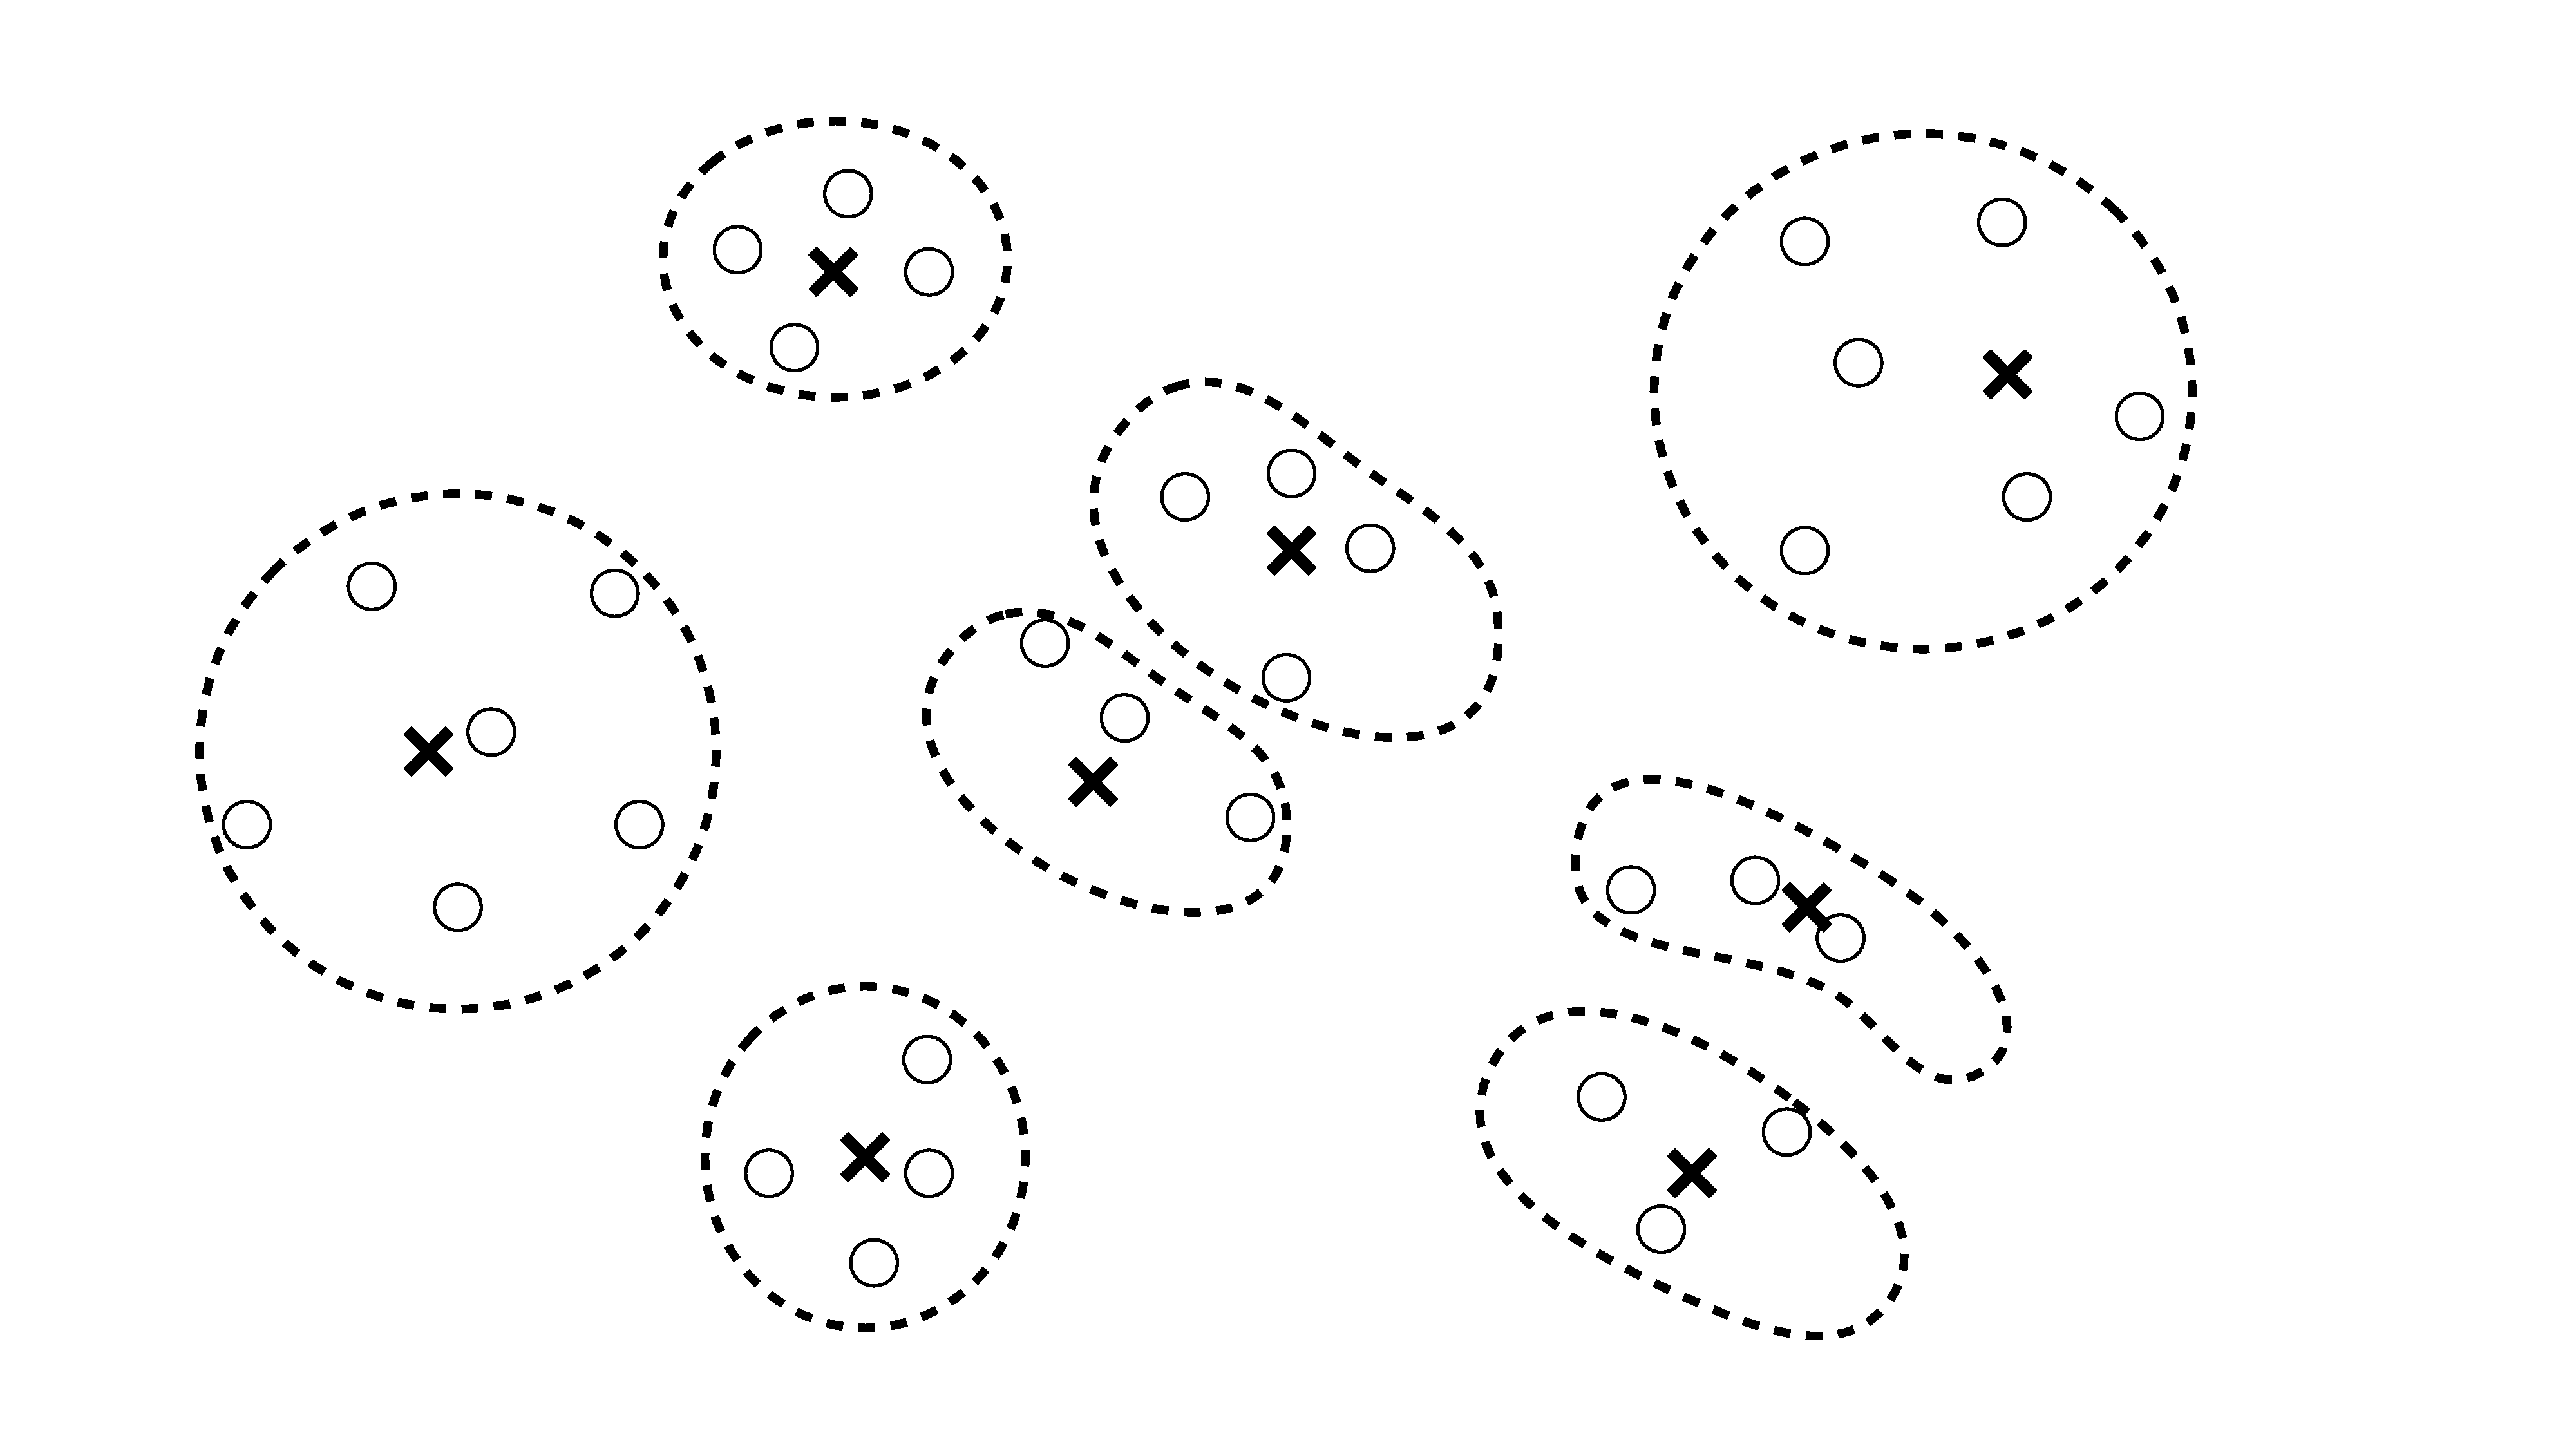
\includegraphics[width=6cm]{pics/chapter2/aid-demo-c.pdf}
    \captionof{figure}{}
    \end{subfigure}
    \caption{\small 聚类拆解步骤示意图}
    \label{aid-demo}

\end{figure}

结合算法2.1,到这里已经给出了完成聚类——迭代拆解最小绝对值回归的所有计算步骤,当聚类无法继续划分时,迭代终止。

下面证明最后一次迭代的解$\hat{\bm{\beta}}_j^T$就是\eqref{l1loss2}的解$\bm{\beta}^*$,
\begin{equation*}
    \begin{split}
        E^* & = \sum_{i \in I} |y_i - \sum_{j \in J}x_{ij}\bm{\beta}j^*|
        = \sum_{k \in K_t}\sum_{i \in C_k^t}|y_i - \sum_{j \in J}x_{ij}\beta_j^*| \\
        & \geq \sum_{k \in K^t}|\sum_{i\in C_k^t}y_i - \sum_{j \in J}x_{ij}\bm{\beta}_j^*|
        = \sum_{k \in K^t}|C_k^t||y_k^t - \sum_{j \in J}x_{kj}^t\bm{\beta}_j^*|\\
        & \geq \sum_{k \in K^t} |C_k^t||y_K^t - \sum_{j\in J}x_{kj} \hat{\bm{\beta}}_j^t|
        = \sum_{k \in K^t} |\sum_{i \in C_k^i} yi - \sum_{i \in C_k^t}\sum_{j \in J}x_{ij}\hat{\bm{\beta}}_j^t| \\
        & = \sum_{k \in k^t} \sum{i \in C_k^i}|y_i - \sum_{j \in J}x_{ij}\hat{\bm{\beta}}_j^t|
        = \sum_{i \in I}|y_i - \sum_{j \in J} x_{ij} \hat{\bm{\beta}}_j^t| 
        = E^t
    \end{split}
\end{equation*}

因为$\hat{\bm{\beta}}_t$是\eqref{l1loss2}的可行解,又显然$E^* \leq E^t$,
这就证明了$E^* = E^t$,注意到$ \sum_{k \in K^t} |C_k^t||y_K^t - \sum_{j\in J}x_{kj} \hat{\bm{\beta}}_j^t|$
就是$F^t$,因此$E^t = F^t$。因此最后一次迭代$F^T$的最优解$\hat{\bm{\beta}}_j^T$就是原问题的最优解。

\subsubsection{优化高维最小绝对值回归}
前面给出的算法已经在很大程度上优化了在处理高维宏观经济变量时,最小绝对值回归计算性能的问题。
而在高维宏观经济实证研究中,变量的维数众多,在建立最小绝对值回归模型时,还需要考虑到变量筛选问题。

对于\eqref{l1losstotal},为了进行变量的筛选,我们需要对估计量$\bm{\beta}^*$的维数做出约束,
一般来说,我们通常采用以下3三种方法:1)$\|\bm{\beta}\|_0 = p$,可以直接选择入选变量的个数;
2)$\|\bm{\beta}\|_2 < s$,该法又称为岭回归;3)$\|\bm{\beta}\|_1 < s$,即为常用的$L_1$正则化方法。
通过加入新的约束,问题的形式也发生了变化。

Park等人于2019年的研究中给出了进一步的结论,对于问题
\begin{equation}\label{l1conclusion}
    E^* = \underset{B\in \phi}{\operatorname{min}} ||Y - f(X, B)||_{L_1}
\end{equation}
其中$Y$为模型响应变量数据矩阵,$X$为解释变量数据矩阵,$B$为模型系数矩阵,$\phi$为模型系数的约束条件。
$f$为任一目标函数,若$f$满足条件
\begin{equation}\label{fcondition}
    f(B, WX) = Wf(B, X)
\end{equation}
其中$W$为一权重矩阵。那么就可以通过聚类——迭代拆解算法求原优化问题的最优解。

而在岭回归和LASSO中,都通过给目标函数加上惩罚项来进行求解,岭回归对应的惩罚项$s\sum_{i=1}^p\bm{\beta}_i^2$,
$L_1$正则化对应的惩罚项为$s\sum_{i=1}^p|\bm{\beta}_i|$,容易发现,加入惩罚项后目标函数仍然满足\eqref{fcondition}
。因此,对于需要进行变量筛选的高维最小绝对值回归问题,我们可以修改目标函数,通过算法2.1解决。

\subsection{一种基于替代变量的估计方法}
聚类——迭代拆解算法是通过有效减少$L_1$目标函数最小化的问题规模来提升求解性能,
每一次迭代仍需要通过线性规划方法求解$L_1$目标函数的最小化问题。
Weidong Liu等人于2020年提出了一种基于替代变量的估计方法,通过替代变量将分位数损失函数转化为$L_2$损失函数,
避免使用线性规划求解分位数损失,因此可以显著提升一般分位数回归的求解性能。

考虑到最小绝对值回归为其特殊情形,且该估计量具有良好的性质,可以在一定程度上解决最小绝对值回归的性能问题。
下面我们介绍如何将该估计应用在最小绝对值回归的场景下,并且给出具体的计算步骤。

\subsubsection{基于替代变量的迭代算法}
考虑\eqref{l1losstotal},
对目标函数稍作形式变换,其中$\rho(x) = x(0.5 - \mathbb{I}[x \leq 0])$,
$\mathbb{I}(x)$为指示函数。
\begin{equation}
\bm{\beta}^* = \underset{\bm{\beta} \in \mathbb{R}^{p}}{\operatorname{arg\ min}}\mathbb{E}|Y - \bm{X}^T\bm{\beta}| = 
\underset{\bm{\beta} \in \mathbb{R}^{p}}{\operatorname{arg\ min}}\mathbb{E}\rho(Y - \bm{X}^T\bm{\beta})
\end{equation}
若已知n\ $i.i.d.$ 的样本$(\bm{X}_i, Y_i)\ (1 \leq i \leq n)$,令$\hat{\bm{\beta}}$为$\bm{\beta}^*$的估计量,则
\begin{equation}\label{rho-problem}
    \hat{\bm{\beta}} = \underset{\bm{\beta} \in \mathbb{R}^{p}}{\operatorname{arg\ min}}\frac1{n}\sum_{i=1}^{n}\rho(Y_i - \bm{X}_i^T\bm{\beta})
\end{equation}

一般地,我们使用牛顿迭代法求解某随机优化问题:
\begin{equation}
    \bm{\beta}^* = \underset{\bm{\beta} \in \mathbb{R}^{p+1}}{\operatorname{arg\ min}} \mathbb{E}[G(\bm{\beta};\bm{X},Y)]
\end{equation}
其中$G(\bm{\beta};\bm{X}, Y)$是损失函数,$\bm{X}$和$Y$分别是$p+1$维自变量和一元响应变量,$\bm{\beta}$为回归系数。使用牛顿-拉弗森迭代来求解,
\begin{equation}
    \tilde{\bm{\beta}}_1 = \bm{\beta}_0 - \bm{H}(\bm{\beta}_0)^{-1}\mathbb{E}[g(\bm{\beta};\bm{X},Y)]
\end{equation}
其中$\bm{\beta}_0$是一个初始估计,$g(\bm{\beta};\bm{X},Y)$为损失函数$G(\bm{\beta};\bm{X},Y)$关于$\bm{\beta}$的梯度。\\
$\bm{H}(\bm{\beta}):=\partial\mathbb{E}[g(\bm{\beta};\bm{X},Y)
/\partial\bm{\beta}$表示$\mathbb{E}G(\bm{\beta};\bm{X},Y)$的海赛矩阵。特别地,我们这里考虑损失函数为$L_1$损失的特殊情形,
\begin{equation}\label{rho-condition}
    G(\bm{\beta};\bm{X},Y) = \rho(Y - \bm{X}^T\bm{\beta})
\end{equation}

在\eqref{rho-condition}的条件下,$g(\bm{\beta};\bm{X},Y) = \bm{X}(\mathbb{I}[Y - \bm{X}^T\bm{\beta} < 0] - 0.5)$。\\
并且,$\bm{H}(\bm{\beta}) = \mathbb{E}(\bm{X}\bm{X}^Tf(\bm{X}^T(\bm{\beta} - \bm{\beta}^*)))$,这里
$f(x)$是噪声$e$的密度函数。当初始估计量$\bm{\beta}_0$和$\bm{\beta}^*$很接近时,$\bm{H}(\bm{\beta}_0)$就会很接近
$\bm{H}(\bm{\beta}^*) = \bm{\Sigma}f(0)$,这里$\bm{\Sigma} = \mathbb{E}\bm{X}\bm{X}^T$是$\bm{X}$的协方差
矩阵。使用$\bm{H}(\bm{\beta}^*)$替换$\bm{H}(\bm{\beta}_0)$,可得

\begin{equation}\label{rho-beta1}
    \bm{\beta}_1 = \bm{\beta}_0 - \bm{H}(\bm{\beta}^*)^{-1}\mathbb{E}[g(\bm{\beta};\bm{X}, Y)]
    = \bm{\beta}_0 - \bm{\Sigma}^{-1}f^{-1}(0)\mathbb{E}[g(\bm{\beta}_0;\bm{X},Y)]
\end{equation}
在$\bm{\beta}^*$对$\mathbb{E}[g(\bm{\beta}_0;\bm{X},Y)$进行泰勒展开,
\begin{equation*}
    \begin{split}
\mathbb{E}[g(\bm{\beta}_0;\bm{X},Y) &= \bm{H}(\bm{\beta}^*)(\bm{\beta}_0 - \bm{\beta}^*) + O(|\bm{\beta}_0 - \bm{\beta}^*|_2^2) \\
 &= \bm{\Sigma}f(0)(\bm{\beta}_0 - \bm{\beta}^*) + O(|\bm{\beta}_0 - \bm{\beta}^*|_2^2)
    \end{split}
\end{equation*}
结合\eqref{rho-beta1},可以得到
\begin{equation*}
    \begin{split}
        |\bm{\beta}_1 - \bm{\beta}^*|_2 &=  |\bm{\beta}_0 - \bm{\Sigma}^{-1}f^{-1}(0)(
            \bm{\Sigma}f(0)(\bm{\beta}_0 - \bm{\beta}^*) + O(|\bm{\beta}_0 - \bm{\beta}^*|_2^2)
        ) - \bm{\beta}^*|_2\\
        &= O(|\bm{\beta}_0 - \bm{\beta}^*|_2^2)
    \end{split}
\end{equation*}
因此,如果我们得到一个$\bm{\beta}^*$的一致估计量$\bm{\beta}_0$,我们就可以通过\eqref{rho-beta1}得到
偏误更小的估计。

下面我们将\eqref{rho-beta1}转化成一个最小二乘问题。首先我们重写该式,
\begin{equation}
    \begin{split}
    \bm{\beta}_1 &= \bm{\Sigma}^{-1}(\bm{\Sigma}\bm{\beta}_0 - f^{-1}(0)\mathbb{E}[g(\bm{\beta}_0;\bm{X},Y)])\\
    &= \bm{\Sigma}^{-1}\mathbb{E}[\bm{X}\{\bm{X}^T\bm{\beta}_0 - f^{-1}(0)(\mathbb{I}[Y \leq \bm{X}^T\bm{\beta}_0] - 0.5)\}]
    \end{split}
\end{equation}
这里我们定义一个新的响应变量$\tilde Y$,
\begin{equation}
    \tilde Y = \bm{X}^T\bm{\beta}_0 - f^{-1}(0) (\mathbb{I}[Y \leq \bm{X}^T\bm{\beta}_0] - 0.5)
\end{equation}
那么$\bm{\beta}_1 = \bm{\Sigma}^{-1}\mathbb{E}(\bm{X}\tilde{Y})$就是线性回归问题$\tilde Y = \bm{X}^T\bm{\beta}$
的最优回归系数,即
\begin{equation}\label{beta1-original}
    \bm{\beta}_1 = \underset{\bm{\beta} \in \mathbb{R}^{p}}{\operatorname{arg\ min}} 
    \mathbb{E}(\tilde Y - \bm{X}^T \bm{\beta})^2
\end{equation}
给定$i.i.d.$样本$(\bm{X}_i, Y_i)$,构造
\begin{equation}\label{svny}
    \tilde{Y}_i = \bm{X}_i^T\hat{\bm{\beta}}_0 - \hat{f}^{-1}(0)
    (\mathbb{I}[Y_i \leq \bm{X}_i^T \hat{\bm{\beta}}_0] - 0.5)
\end{equation}
其中$\hat{\bm{\beta}}_0$为$\bm{\beta}^*$的一个初始估计,$\hat{f}(0)$为$f(0)$的一个估计
\begin{equation}\label{yl2loss}
    \hat{\bm{\beta}} = \underset{\bm{\beta} \in \mathbb{R}^{p}}{\operatorname{arg\ min}}
    \frac1{n} \sum_{i=1}^n(\tilde{Y}_i - \bm{X}_i^T\bm{\beta})^2
\end{equation}
这里我们选择某估计量作为$\hat{\bm{\beta}}_0$,并且采用$f(0)$的核密度估计作为$\hat{f}(0)$,

$$
    \hat{f}(0) = \frac1{nh}\sum_{i=1}^nK(\frac{Y_i - \bm{X}^T_i\hat{\bm{\beta}}_0}{h})
$$
其中$K(x)$为核函数,$h \rightarrow 0$是带宽,本方法对待估系数的稀疏性有较强的要求(Weidong Liu,2020),并且
在每次迭代都需要调整带宽。

只要给定的初始值$\hat{\bm{\beta}}_0$是$\bm{\beta}^*$的一致估计量,那么$\hat{\bm{\beta}}$就将会是一个更加接近
$\bm{\beta}^*$的新的估计,并且\eqref{yl2loss}为最小二乘问题,其计算十分简便。

我们当然可以将$\hat{\bm{\beta}}$作为\eqref{rho-beta1}的初始值,这样继续构造替代变量进行迭代,最终收敛到$\bm{\beta}^*$。
算法2给出了使用替代变量估计方法的计算步骤。
\begin{table}[H]%%%%%%开始表格
    \centering%把表居中
    \begin{tabular}{{p{0.9\columnwidth}}}%三个c代表该表一共三列,内容全部居中
    
    \toprule%第一道横线 表头
    算法2.2 使用替代变量迭代算法方法求解最小绝对值回归问题(SVN, substitue variable newton method)\\
    \midrule%第二道横线 符号+解释+单位 中间用&隔开
    输入:$Y$和$\bm{X}$的样本$\bm{Y} = (Y_1, Y2, ..., Y_n)$,$\bm{X} = (\bm{X}^T_1, \bm{X}^T_2, ..., \bm{X}^T_n)$,
    迭代次数$T$,核函数$K$,依赖于迭代次数的带宽$h_t(t = 1, ..., T)。$
    \\
    初始化:给出初始相合估计量,$\hat{\bm{\beta}}^{(0)} $,将样本划分成$J$个均等子集,样本量均为$m$,为了给出最小绝对值回归估计量的相合估计,
    我们取任一子集里面的数据,直接使用最小一乘法估计$\hat{\bm{\beta}}_{(0)}$。
    \\
    对于$t = 1, ..., T$:
    取新的数据子集,在该数据集上
    \\
        1. 计算$\hat{f}^{t}(0)$,
        $$
        \hat{f}^{t}(0) = \frac1{mh}\sum_{i=1}^{m}K(\frac{Y_i - \bm{X}_i^T\hat{\bm{\beta}}^{t-1}}{h_t})
        $$
    \\
        2. 计算$\tilde{Y} = (\tilde Y_1, \tilde Y_2, ..., \tilde Y_m)$,
        $$
        \tilde{Y}_i = \bm{X}^T_i\hat{\bm{\beta}}^{t-1} - \hat{f}^{t}(0)^{-1}
        (\mathbb{I}[Y_i \leq \bm{X}_i^T \hat{\bm{\beta}}^{t-1}] - 0.5)
        $$
    \\
        3. 计算$\hat{\bm{\beta}}^{t}$,
        $$
        \hat{\bm{\beta}}^{t} = \underset{\bm{\beta} \in \mathbb{R}^{p}}{\operatorname{art\ min}}
        \frac1{m}\sum_{i=1}^m (\tilde{Y}_i - \bm{X}_i^T\bm{\beta})^2
        $$
    \\
    输出:$\bm{\beta}^{(T)}$
    \\
    \bottomrule%第三道横线
    \end{tabular}
\end{table}%%%%%%结束表格

\subsubsection{优化高维最小绝对值回归}
在高维相依自变量的情形下,我们只需在\eqref{beta1-original}加入惩罚项即可,例如我们使用$L_1$正则化,那么
\begin{equation}
    \bm{\beta}_{1, \lambda} =\underset{\bm{\beta} \in \mathbb{R}^{p}}{\operatorname{arg\ min}} 
    \mathbb{E}(\tilde Y - \bm{X}^T \bm{\beta})^2 + \lambda|\bm{\beta}|
\end{equation}
对应的,最终估计量计算如下
\begin{equation}\label{beta1-lasso}
    \hat{\bm{\beta}} = \underset{\bm{\beta} \in \mathbb{R}^{p}}{\operatorname{arg\ min}}
    \frac1{n} \sum_{i=1}^n(\tilde{Y}_i - \bm{X}_i^T\bm{\beta})^2 + \lambda|\bm{\beta}|
\end{equation}
\eqref{beta1-lasso}是著名的LASSO问题,已经有了快速解决的算法。因此,对于高维情形,算法2仅需稍作改动。

\subsection{模拟实验}
本章前面两节介绍了聚类——迭代拆解算法和一种基于替代变量的迭代算法,
前者通过减小问题规模、逐步逼近最优解的方法来提升计算性能,
而后者通过变量替换的方法将最小绝对值回归问题转化为最小二乘问题,在给定一个相合估计条件下逼近最优解。
两种方法都可以处理带有惩罚项和不带有惩罚项的最小绝对值回归问题,并且我们已经给出了各自计算的具体步骤。

本节将通过一个数值模拟实验来比较和分析两种方法的性能表现,分析其优缺点。

\subsubsection{数据准备}
设定模拟数据来自下面的模型:
\begin{equation*}
    {Y}_i = \bm{X}_i^T \bm{\beta} + e_i, i = 1, 2, ..., n
\end{equation*}
其中$\bm{X}_i = (1, X_{i,1}, ..., X_{i, p-1})$为$p$维随机向量,
在比较不带惩罚项的最小绝对值回归的场合,令$X_i$的各维度服从独立同分布。
我们设置不同$p, n$的组合用来测试算法的计算性能,并观察在不同的噪声分布下,估计结果的准确性。
对于系数$\bm{\beta}$,设$s$为其$L_0$范数,取
$$
    \bm{\beta} = (\frac{10}{s}, \frac{20}{s}, ..., \frac{10(s-1)}{s}, 10, 0, ..., 0)
$$

对于算法2.1,以下简称SVN的每步最佳带宽依赖于数据集的性质,参考weidong liu等,这里给出
$$
    h^t = \sqrt{\frac{s\log n}{n}} + s^{-1/2} (\frac{s^2\log n}{10m})^{(t+1)/2},
$$
核函数选取高斯核函数。

对于聚类——迭代拆解算法,我们这里选择初始聚类方法如下:
首先从原始数据中少量采样(本实验取$max\{0.5\%n, m\}$),通过最小绝对值回归给出系数估计$\bm{\beta}^{init}$,
对每一个原始数据点,计算其在当前模型系数下的残差,然后进行K-means聚类得到$C^0$。

本次实验对比基准使用线性规划内点法(以下简称LP)求解。我们给出了SVN算法和AID算法的Python3实现,数值计算基于numpy包,
作为基准的LP使用Scipy数值计算包的对应实现。

\subsubsection{实验结果}

我们采用最终估计值和真实值差的$L_2$范数来衡量准确性。
在实验结果中中我们着重观察算法的收敛性、算法的准确性和计算性能。

我们在高斯噪声下,比较三种算法的性能表现。

表\ref{tab-performance}中,$r^0$表示AID算法初始聚类$K_0/n$的值,而$r^T$表示算法终止时$K_T/n$的取值。
需要注意的是,对于AID算法,$T$表示算法终止时经历的迭代次数,$Time$表示算法终止时运算的cpu时间。
而对于SVN算法,$T$表示其每估计值达到稳定的迭代次数,$Time$表示全部数据参与迭代完毕经历的cpu时间。
\begin{table}[H]
    \centering
    \begin{tabular}{@{}ccccccccc@{}}
    \toprule
           &     & \multicolumn{4}{c}{AID}        & \multicolumn{2}{c}{SVN} & LP        \\ \midrule
    n      & m   & $r^0$(\%) & $r^T$(\%) & T  & Time(sec) & T      & Time(sec)      & Time(sec) \\ \midrule
    20000  & 10  & 0.05  & 2.90  & 6  & 2         &  3      &         0.38       & 0.20      \\
    20000  & 50 & 0.15  & 12.00 & 12 & 13        &   7     &          6     & 3       \\
    20000  & 100 & 0.15  & 12.00 & 12 & 38        &  11      &         27    & 21         \\
    20000  & 200 & 0.66  & 21.55 & 9  & 118        &   8     &          76      & 126        \\
    20000  & 500 & 0.80  & 28.00 & 11 &  535      &  3      &              322  &     813 \\ 
    40000  & 10  & 0.05  & 2.90  & 6  & 3        &  3      &         0.74      & 0.23     \\
    40000  & 50 & 0.15  & 12.00 & 12 & 31        &   7     &          14     & 7       \\
    40000  & 100 & 0.15  & 12.00 & 12 & 84       &  8      &         56    & 48         \\
    40000  & 200 & 0.66  & 21.55 & 9  & 210        &   8     &          154     & 258        \\
    40000  & 500 & 0.80  & 28.00 & 11 & 1965       &  3      &             1143   &  3446      \\ 
    200000  & 100 & 0.80  & 11.00 & 11 & 134       &  3      &          361      &   496     \\ 
    200000  & 200 & 0.80  & 28.00 & 11 & 2476       &  3      &          1631      &   3329     \\ 
    \bottomrule
    \end{tabular}
    \caption{\small 高斯噪声下三种估计算法的性能比较。(处理机情况:苹果M1芯片8核,8GB内存,OSX,CPython解释器3.82Arm版)}
    \label{tab-performance}
\end{table}

可以看出在$n,m$较大场合下,AID算法和SVN算法均在性能上有领先,尤其是SVN算法具有优异的性能表现。

\begin{figure}[H]
    \centering
    \begin{subfigure}[t]{0.3\textwidth}\label{svn-demo1}
    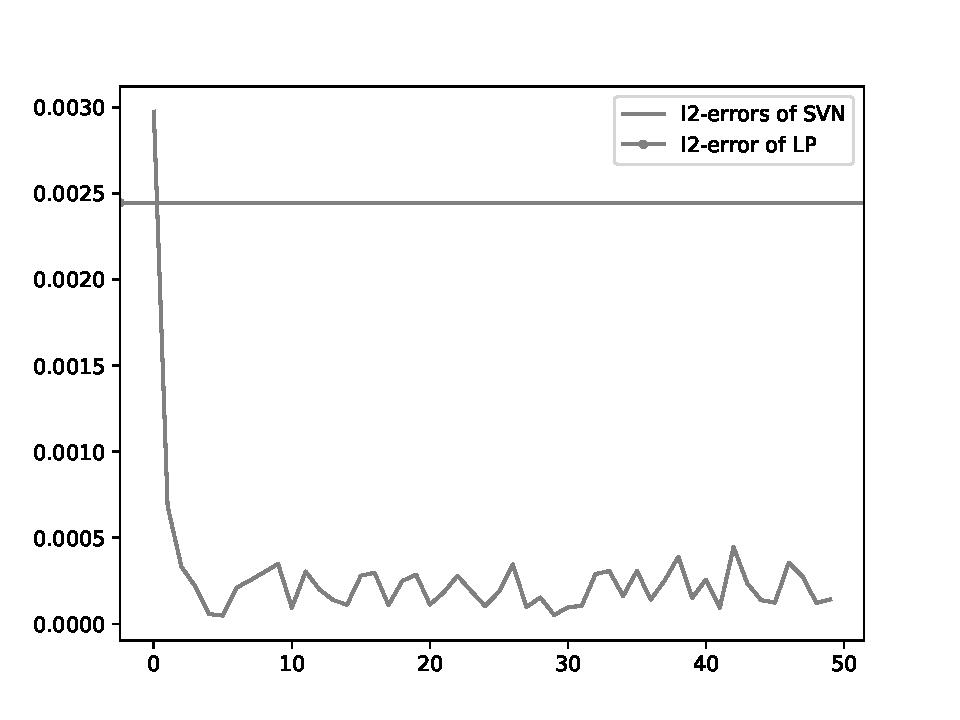
\includegraphics[width=5cm]{pics/chapter2/svn-l2.pdf}
    \captionof{figure}{}
    \end{subfigure}
    \begin{subfigure}[t]{0.3\textwidth}\label{svn-demo2}
    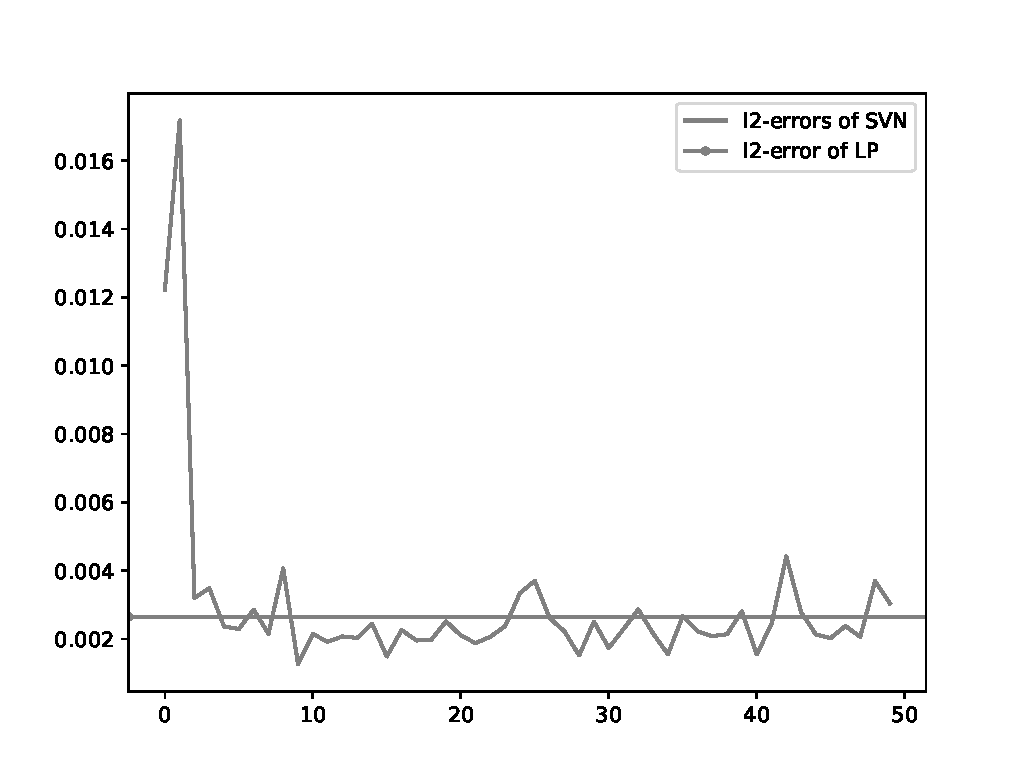
\includegraphics[width=5cm]{pics/chapter2/svn-l2-3.pdf}
    \captionof{figure}{}
    \end{subfigure}
    \begin{subfigure}[t]{0.3\textwidth}\label{svn-demo3}
    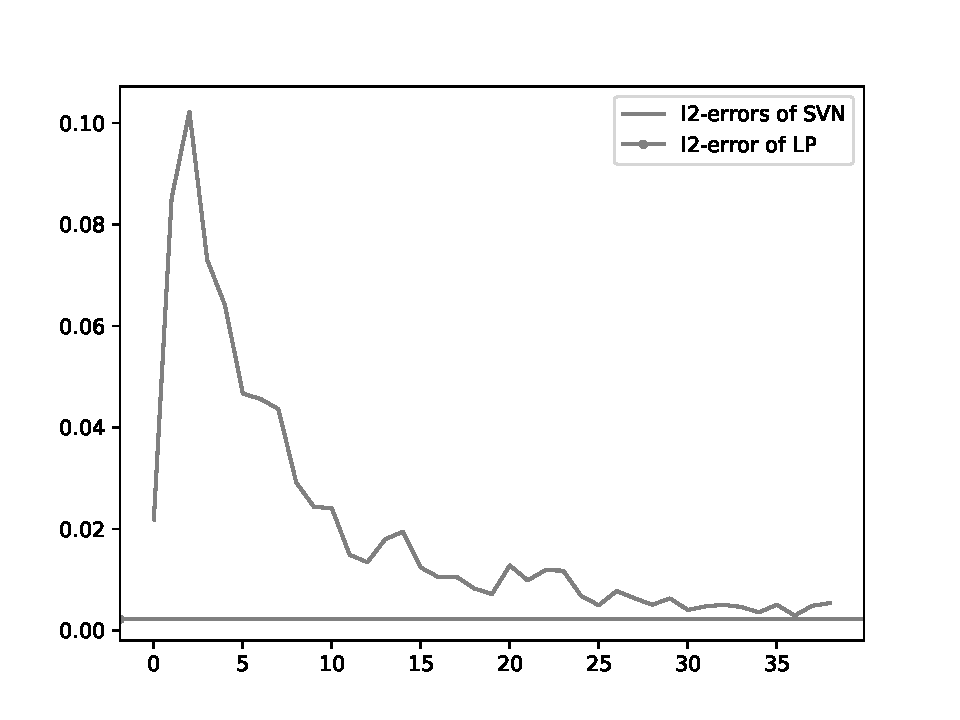
\includegraphics[width=5cm]{pics/chapter2/svn-conver.pdf}
    \captionof{figure}{}
    \end{subfigure}
    \caption{ \small SVN算法的迭代情况图。横轴代表了迭代次数,纵轴代表了估计的误差平方和。(a)中$n=20000,p=10,s=4$,(b)中$n=20000,p=50,s=20$,
    (c)中$n=20000,p=100,s=80$。}
    \label{svn-demo}

\end{figure}

图\ref{svn-demo}展示了SVN算法出色的收敛速度。我们观察到SVN算法在系数具有稀疏性时表现明显更好,这也符合该算法提出的理论基础。
我们可发现,在稀疏条件下,SVN算法在很快趋近平稳;在系数不具有系数性时,SVN算法准确度明显降低,并且收敛速度变慢。
然而大多数的情况下,对于常见的宏观经济线性模型,系数稀疏的现象更加普遍。在稀疏的条件下,SVN算法表现出了十分出色的性能和估计精确度,需要
注意的是在样本充分大的情况下,我们不需要将划分的每一组数据纳入计算,在能够使得估计量取值稳定的有限步骤内返回即可,这时SVN算法的计算时间还可以进一步缩短。

接下来我们观察不同噪声分布的影响,由于AID算法和线性规划方法具有同样的解,图\ref{svn-noise}给出了不同的噪声分布下SVN算法的表现,
可以看到,由于SVN算法并没有直接使用$L_1$损失,其在面对柯西噪声这种重尾的极端情况下精度不如直接优化$L_1$损失的算法。

\begin{figure}[H]
    \centering
    \begin{subfigure}[t]{0.3\textwidth}\label{svn-demo1}
    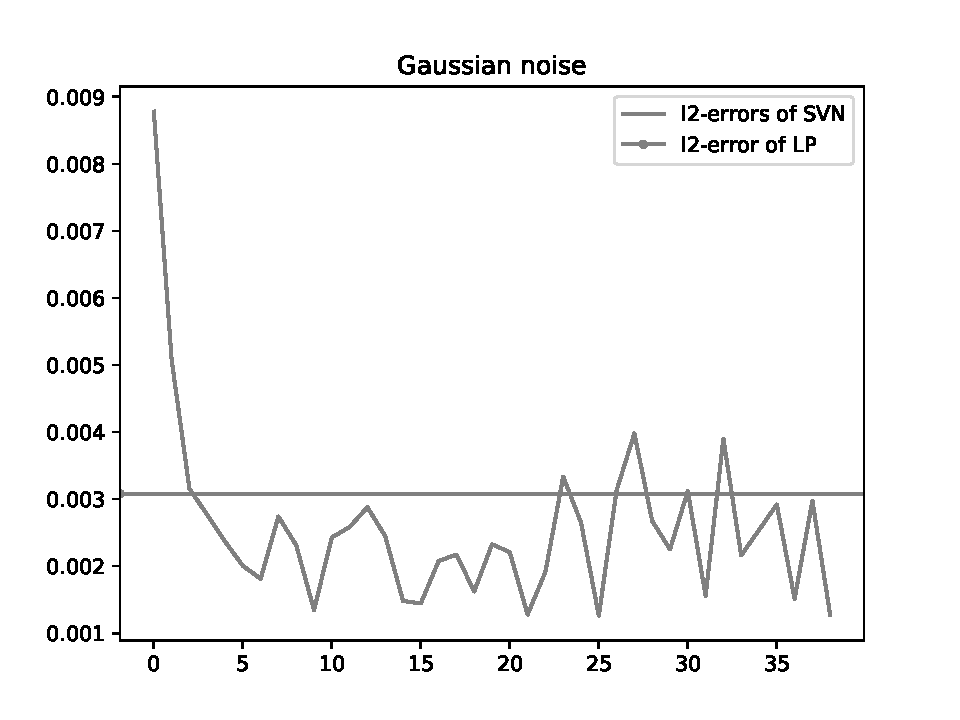
\includegraphics[width=5cm]{pics/chapter2/gauss.pdf}
    \captionof{figure}{}
    \end{subfigure}
    \begin{subfigure}[t]{0.3\textwidth}\label{svn-demo2}
    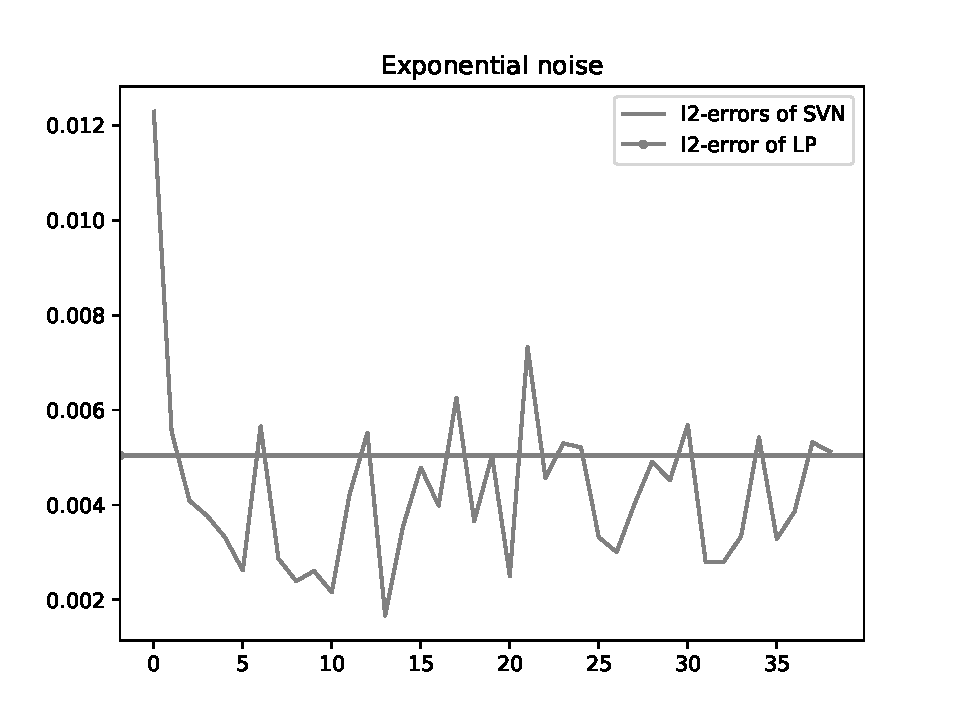
\includegraphics[width=5cm]{pics/chapter2/expential.pdf}
    \captionof{figure}{}
    \end{subfigure}
    \begin{subfigure}[t]{0.3\textwidth}\label{svn-demo3}
    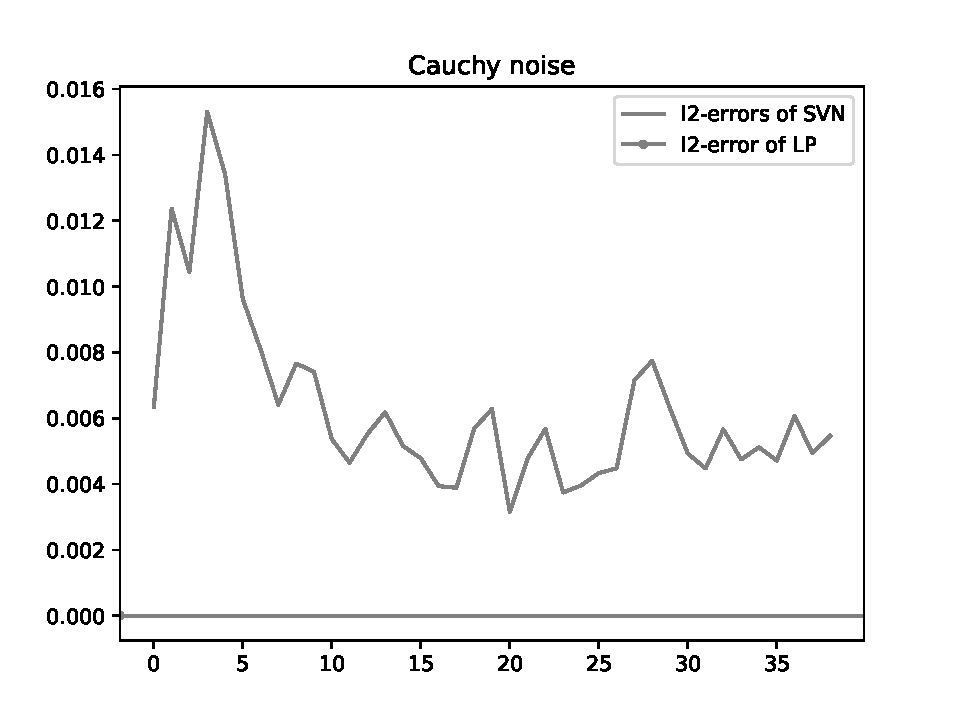
\includegraphics[width=5cm]{pics/chapter2/cauchy.pdf}
    \captionof{figure}{}
    \end{subfigure}
    \caption{ \small SVN算法在各种噪声下的表现。$n=20000,p=50,s=20$}
    \label{svn-noise}

\end{figure}

而AID算法虽然在计算时间上并没有SVN算法表现出色,但是它的确在大规模数据下减少了计算量。并且AID算法可以保证获得最优解,
这是SVN算法不具备的优势;另外,SVN算法的准确度和带估系数的稀疏性紧密相关,在高维非稀疏的场合下,SVN算法并不具备很好的准确性。

考虑到在加入惩罚项后,AID算法和LP需要解决增加该额外约束的线性规划问题,其计算复杂度将上升。
而SVN算法,需要求解\eqref{beta1-lasso},目前已有的LASSO算法可以快速求解。
因此SVN算法在带有$L_1$惩罚项的场景下,更加体现其性能优势,因此本节不再赘述。


\subsection{本章小结}

本章首先简要介绍了$L_1$范数的概念,列举了一些其在经济数据分析领域的应用。随后,讨论了
最小绝对值回归的稳健性和其求解方法。

最小绝对值回归已经广泛应用在高维宏观经济数据的处理中,但是它在应用中存在一定的性能问题。
本章介绍了两种可以应用于最小绝对值回归的优化手段:聚类——迭代拆解算法和基于替代变量的估计方法。
进行了数值模拟实验,分析了其优缺点,并给出了其在实际应用中的几点建议。

聚类——迭代拆解算法
是一种非常好的思想,它结合了机器学习中聚类的方法,聚类的作用可以将信息进行提纯,在经过处理
后的数据集上解决原始问题对应的加权优化问题,可以避免直接解决原始问题而耗费庞大的计算量。
聚类——迭代拆解算法可以应用于解决最小绝对值回归问题,它在一定程度上减少了线性规划的计算量,
并且在理论上具有最优解,即它的解一定可以和直接对所有数据求解进行线性规划问题一样好。

另外,本章介绍了另外一种巧妙的算法——一种基于替代变量的迭代算法,该算法通过
构造替代变量,从而将原来需要通过线性规划解决的最小绝对值回归问题转化为
解决替代变量的最小二乘问题。这样一来,计算的复杂度就大大降低。该方法在
实际系数具有系数性时表现十分优秀。

这两种算法都可以在特定的条件下,优化最小绝对值回归的计算速度。
目前高维宏观经济数据分析中也经常使用最小绝对值回归进行某些计算,
我们可以根据数据的规模和问题的特点来选择以上两种方法来代替线性规划。

最后,我们在本章对最小绝对值回归性能优化的研究,会对之后
章节对$L_1$范数主成分分析的应用研究有推动作用。
